\section{Les gestionnaires de versions}
\begin{frame}
  \tableofcontents[sectionstyle=show/shaded]
\end{frame}

\usebackgroundtemplate{}

\begin{frame}{Moyens primitifs}
Gérer un projet de programmation sans gestionnaire de versions :
\begin{itemize}
  \item S'envoyer l'entièreté du code par mail ;
  \item Partage de fichiers sur un serveur (dropbox, …) ;
  \item S'envoyer des \textit{patchs} :
  \begin{itemize}
    \item commande \texttt{diff} : différence entre deux fichiers/dossiers ;
    \item commande \texttt{patch} : appliquer le \textit{patch} (la \textit{diff}).
  \end{itemize}
  \item etc.
\end{itemize}

\pause
\bigskip
Pas très pratique !
\end{frame}

\begin{frame}{Buts d'un gestionnaire de versions}
  \begin{itemize}
    \item Faciliter la gestion d'un projet de programmation ;
    \item Garder l'historique de toutes les modifications (\textit{commits}) ;
    \item Travailler en équipe ;
    \item Avoir des branches de développement :
      \begin{itemize}
        \item pour développer une fonctionnalité séparément ;
        \item pour une certaine version (2.4.0 $\rightarrow$ 2.4.1 $\rightarrow$ ...).
      \end{itemize}
  \end{itemize}

  \bigskip
  \begin{center}
    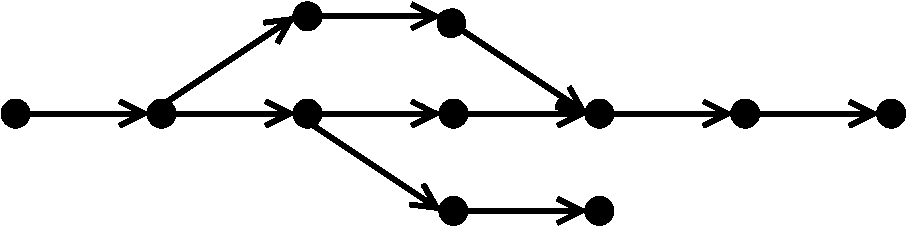
\includegraphics[scale=0.4]{commit-branch.pdf}
  \end{center}
\end{frame}

\begin{frame}{Micro-commits}
  Un \textit{commit} = \textbf{une} modification bien particulière

  \bigskip
  Avantages :
  \begin{itemize}
    \item Plus facile à comprendre pour les autres
    \item Possibilité d'annuler un changement facilement (\texttt{git revert})
    \item Trouver l'origine d'un bug (\texttt{git bisect})
    \item …
  \end{itemize}
\end{frame}

% He who controls the version control, controls the past.

\begin{frame}{Historique des gestionnaires de versions}
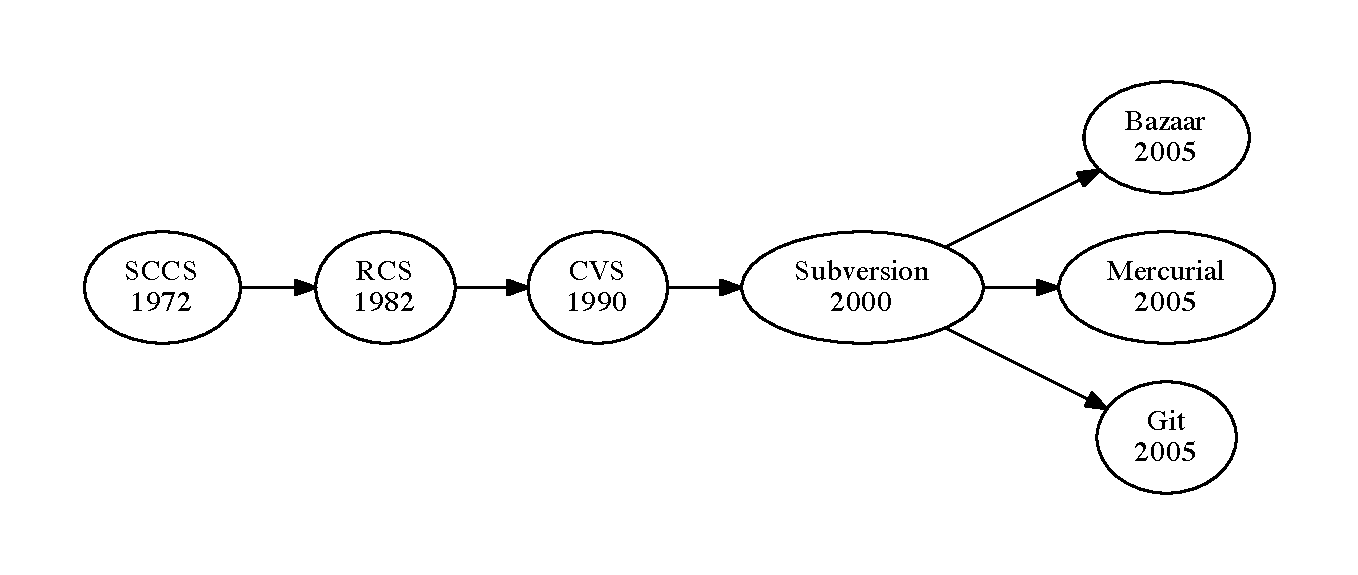
\includegraphics[width=\textwidth]{vcs-history.pdf}
\end{frame}

\begin{frame}{Subversion}
  Subversion (SVN) est \textbf{centralisé} :
  \begin{itemize}
    \item Un serveur central contient toutes les données ;
    \item Beaucoup de requêtes entre le client et le serveur (assez lent) ;
    \item Besoin d'une connexion internet pour travailler.
  \end{itemize}
\end{frame}

\begin{frame}{Git}
  Git est \textbf{décentralisé}/\textbf{distribué} :
  \begin{itemize}
    \item Toutes les données sont sur notre machine ;
    \item Les opérations sont très rapides ;
    \item Connexion internet seulement pour les \textit{pull} et \textit{push}.
  \end{itemize}

  \pause
  \bigskip
  Git est aussi \textbf{plus puissant} et \textbf{plus flexible} :
  \begin{itemize}
    \item Pour la gestion des branches ;
    \item Possède de nombreuses fonctionnalités plus avancées.
  \end{itemize}
\end{frame}

\begin{frame}{Serveur central avec Git}
  \begin{itemize}
    \item Une manière simple de travailler en équipe ;
    \item Accès en écriture pour tous les développeurs.
  \end{itemize}

  \bigskip
  \begin{center}
    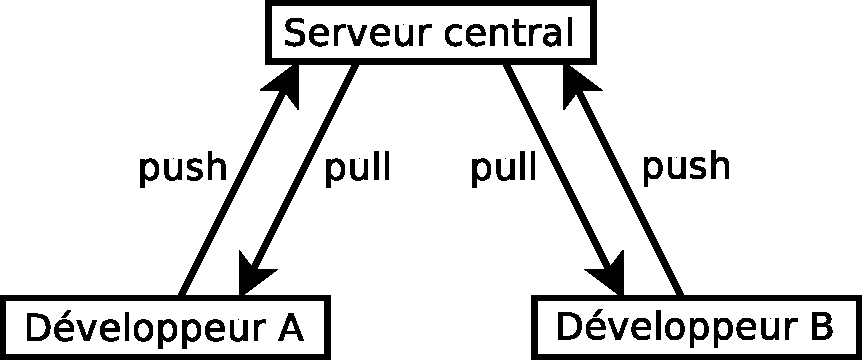
\includegraphics[scale=0.5]{pull-push-central-server.pdf}
  \end{center}
\end{frame}

\begin{frame}{Git est décentralisé}
  \begin{itemize}
    \item Seul les mainteneurs ont accès en écriture ;
    \item Les contributeurs font des \textit{pull requests}.
  \end{itemize}

  \bigskip
  \begin{center}
    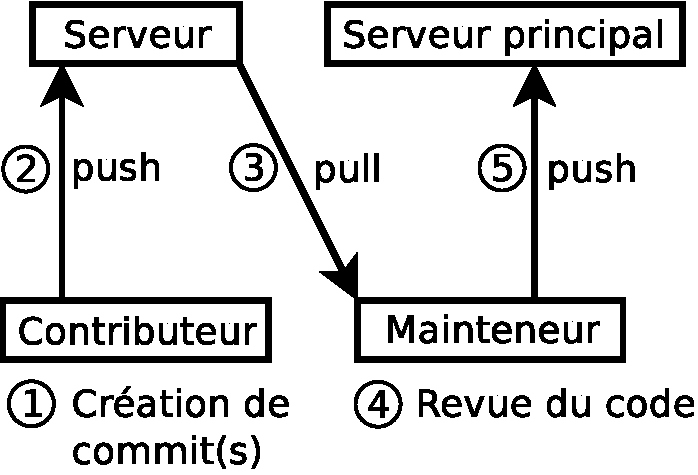
\includegraphics[scale=0.5]{pull-push-distributed.pdf}
  \end{center}
\end{frame}
